
\section*{Instrucciones de la práctica}
El alumno deberá entregar un archivo bfs secuencial.py que contendrá una implementación de BFS para gráficas. Su función deberá recibir la gráfica \(A\) como argumento, (que empiece por el nodo A pero si se hace el punto extra de que en terminal una gráfica cualquiera se puede mandar, en
el programa se debe de empezar desde el nodo que sea) y deberá regresar una lista de los nodos visitados.
Su programa debe funcionar para gráficas conexas.

\begin{figure}[h]
	\centering
	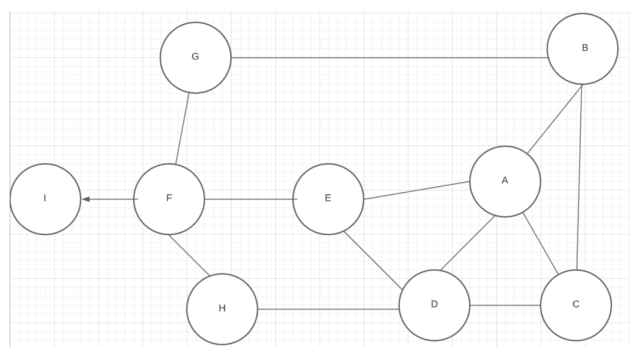
\includegraphics[width=0.7\textwidth]{images/gA.png}
	\caption[grafica A]{Gráfica A}
\end{figure}

\section*{Razonamiento}
Representar una gráfica en código puede hacerse de muchas formas, unas más ineficientes que otras, como podría ser con una matriz de adyacencias, pero nosotros decidimos usar una opción más eficiente y común, una lista de adyacencias.

Lo anterior conste en tener una lista de con los nodos de la gráfica, y para cada uno de estos, otra lista que indicará con que nodos está conectado el nodo. 

Es posible programarla directamente con listas de listas, pero más eficiente sería usar un diccionario de diccionarios o un diccionario de listas, ya que esto mejora la complejidad para acceder a los nodos. En nuestro caso usamos un diccionario de listas, ya que realmente solo vamos a recorrer la gráfica con BFS y no revisar adyacencias de los nodos. 

Recordemos que el agoritmo de BFS para gráficas se basa en empezar desde un nodo \(v\) y seguir con sus vecinos, luego con los vecinos de los vecinos y así sucesivamente hasta recorrer todos los nodos de la gráfica. Pero dado que estámos trabajando con gráficas simples, lo anterior facilmente podría producir un problema pues si tenemos el nodo \(v\) que es vecino de \(u\), entonces \(u\) tiene como vecino también a \(v\) y esto podría producir un ciclo, entonces necesitamos una forma de poder marcar a los nodos que ya fueron visitados para no volverlos a visitar.

Entonces nuestras gráficas también contaran con un diccionario con sus nodos que indicará si un nodo ya fue visitado o no, y para ello lo marcaremos con un valor booleano. 

Y para implementar BFS podemos hacerlo de forma recursiva o iterativa, pero se nos hizo más sencillo hacerlo iterativo. 
Entonces, una estuctura que justo nos ayuda a modelar lo principal del algoritmo (recorrer primero los vecinos de un nodo, y luego los vecinos de esos vecinos) es una cola, pues sigue el principio de que el primer elemento que entra es el primero que sale, por lo tanto, si nosotros metemos un nodo \(v\) a la cola, y al sacarlo lo marcamos como visitado (para no visitarlo después) y metemos a todos los vecinos de \(v\) a la cola, nos aseguramos de que los siguientes elementos que salgan de la cola sean los vecinos de \(v\), y luego los vecinos de esos vecinos, y así sucesivamente, siguiendo el orden deseado.


\section*{Consideraciones}
Algunas consideraciones extra que tuvimos que tener en cuenta fueron las excepciones que maneja el programa, principalmente aquellas que tienen que ver con las gráficas validas que podemos aceptar.

Nosotros consideramos como una gráfica valida a aquellas que tienen al menos un nodo, y que su número de aristas no rebasa \(\dfrac{n(n-1)}{2}\) (pues ese es el número de aristas máximas en una gráfica con \(n\) nodos). También estamos interesados en que la gráfica sea conexa, pues de no ser así, no se podría ejecutar \(BFS\) en cualquier nodo y obtener un recorrido que pase por todos los nodos de la gráfica. 